\begin{figure}
	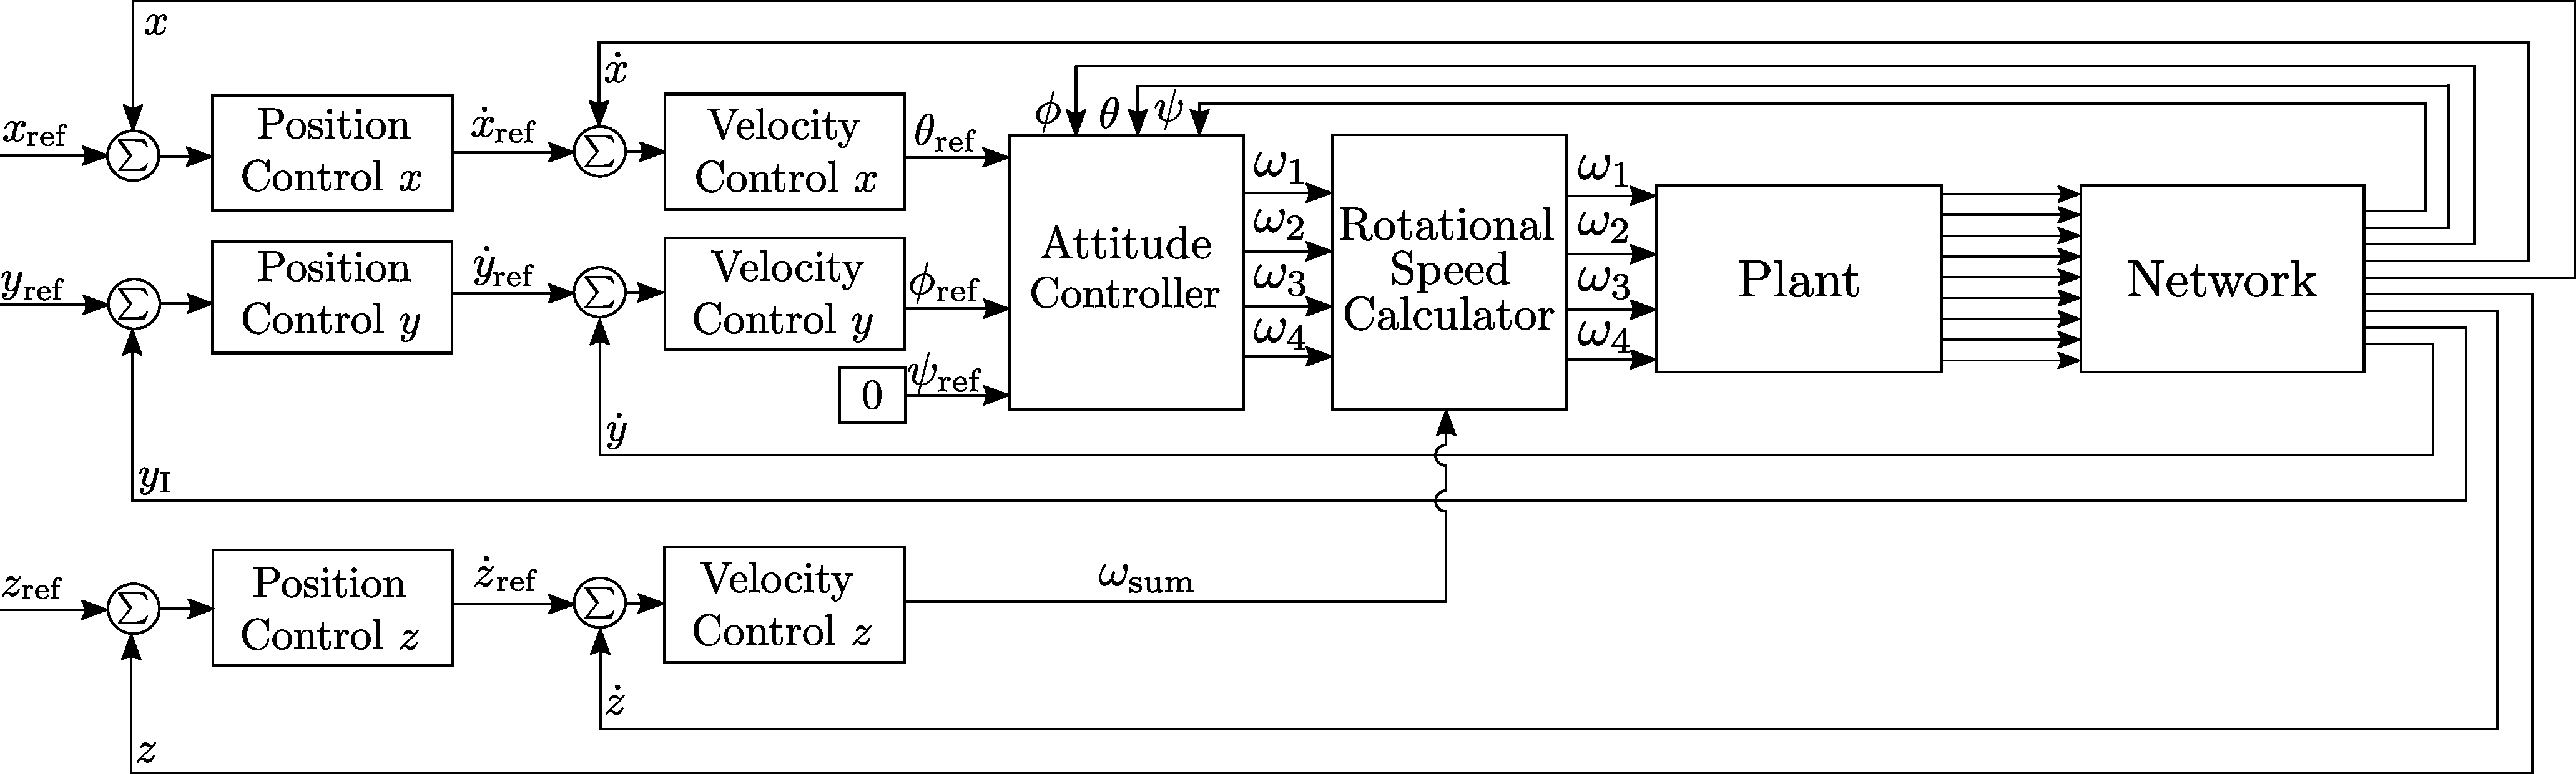
\includegraphics[width=0.7\linewidth]{figures/TranslationalControlDiagram}
	\caption{Figure caption}
\end{figure}


\begin{columns}[t,totalwidth=\twocolwid] % Split up the two columns wide column
	
	\begin{column}{0.46\twocolwid} % The first column within column 2 (column 2.1)
		 \begin{itemize}
			\item Attitude controller\\
			State feedback with integral control, to be able to track references and handle disturbances, is used along with a reduced order observer, estimating angular velocities.
		\end{itemize}
	\end{column} % End of column 2.1
	
	\begin{column}{0.46\twocolwid} % The second column within column 2 (column 2.2)
		 \begin{itemize}
			\item Translational controller\\
			PI controller are used to control the translational velocities.\\
			Bandwidth of the cascaded controllers need to be taken into account in order to reduce the effect.
		\end{itemize}		
	\end{column} % End of column 2.2
	
\end{columns} % End of the split of column 2 - any content after this will now take up 2 columns width